\documentclass[xcolor={dvipsnames}]{beamer}

%%% PACKAGES %%%
\usepackage{graphicx}
\usepackage{tabularx}
\usepackage{booktabs}
\usepackage{multirow}
%\usepackage[usenames,dvipsnames]{color}
\usepackage{textpos}
\usepackage{tipa}
\usepackage{hyperref}
%\usepackage{pifont}



%%% FONT %%%
\usepackage{tgheros}


%%% BEAMER THEME %%%
\usetheme{default}
\usecolortheme{whale}
\usecolortheme{orchid}
\setbeamertemplate{navigation symbols}{} 
\setbeamertemplate{footline}[frame number]
%\setbeamertemplate{footline}{%
%  \leavevmode%
%  \hbox{%
%    \pgfsetfillopacity{0}\begin{beamercolorbox}[wd=.333333\paperwidth,ht=2.25ex,dp=1ex,center]{author in head/foot}%
%      \usebeamerfont{author in head/foot}\pgfsetfillopacity{1}\insertshortauthor
%    \end{beamercolorbox}%
%    \pgfsetfillopacity{0}\begin{beamercolorbox}[wd=.333333\paperwidth,ht=2.25ex,dp=1ex,center]{title in head/foot}%
%      \usebeamerfont{title in head/foot}\pgfsetfillopacity{1}\insertshorttitle
%    \end{beamercolorbox}%
%    \pgfsetfillopacity{0}\begin{beamercolorbox}[wd=.333333\paperwidth,ht=2.25ex,dp=1ex,right]{date in head/foot}%
%      \usebeamerfont{date in head/foot}\pgfsetfillopacity{1}\insertshortdate{}\hspace*{2em}
%      \insertframenumber{} / \inserttotalframenumber\hspace*{2ex}
%    \end{beamercolorbox}}%
%  \vskip0pt%
%}
\addtobeamertemplate{frametitle}{}{%
\begin{textblock*}{100mm}(.875\textwidth,-1cm)

\includegraphics[height=1cm]{../../../img/uni_des_saarlandes-white.png}
\end{textblock*}}
\setbeamertemplate{caption}{\insertcaption}
\setbeamerfont{caption}{size=\scriptsize}
\setbeamertemplate{itemize subitem}[circle]
%\setbeamertemplate{bibliography item}[text]
\setbeamertemplate{bibliography item}[triangle]
\setbeamertemplate{blocks}[rounded][shadow=true]


%%% COLORS %%%
\definecolor{MutedBlue}{RGB}{83,121,170}
\definecolor{UniBlue}{RGB}{0,71,116}
\definecolor{DarkPink}{RGB}{178,56,119}
\definecolor{LightPink}{RGB}{255,224,246}
\definecolor{LightBlue}{RGB}{214,255,255}

%\setbeamercolor{title}{fg=UniBlue}
%\setbeamercolor{frametitle}{fg=UniBlue}
\setbeamercolor{author in head/foot}{fg=UniBlue}
\setbeamercolor{title in head/foot}{fg=UniBlue}
\setbeamercolor{date in head/foot}{fg=UniBlue}
\setbeamercolor{page number in head/foot}{fg=UniBlue}
\setbeamercolor{normal text}{fg=darkgray}
\setbeamercolor{structure}{fg=UniBlue}
\setbeamercolor{itemize item}{fg=UniBlue}
\setbeamercolor{itemize subitem}{fg=UniBlue}
%\setbeamercolor{section in toc}{fg=MutedBlue}
%\setbeamercolor{subsection in toc}{fg=darkgray}
%\setbeamercolor{bibliography entry author}{fg=darkgray}
%\setbeamercolor{bibliography entry title}{fg=darkgray}
%\setbeamercolor{bibliography entry location}{fg=gray!80!black}
%\setbeamercolor{bibliography entry note}{fg=gray!90!black}
%\setbeamercolor{bibliography entry note}{fg=darkgray}
\setbeamercolor{block title}{bg=structure,fg=white}
%\setbeamercolor{block body}{bg={palette secondary}}


%%% FOOTNOTES %%%
\usepackage{perpage}
\MakePerPage{footnote} %restart numbering on each slide
\renewcommand{\footnotesize}{\scriptsize}

%%% BIBLIOGRAPHY %%%
\usepackage[%
	backend=bibtex,
	citestyle=authoryear,
	maxcitenames=2,
	maxbibnames=99,
	firstinits=true,
	url=false,
	doi=false,
	isbn=false, 
	%sorting=none,
	]{biblatex}
\addbibresource{../slaterefs.bib}
% use \footfullcite{jones00}

%% TITLE PAGE INFO %%
\author[A. Vakil \& J. Trouvain]{Anjana Vakil and J\"{u}rgen Trouvain
%\\\texttt{[anjanav,trouvain]@coli.uni-saarland.de}
} 
\institute{
\includegraphics[height=4.5em]{../../../img/uni_des_saarlandes.png}\\Department of Computational Linguistics and Phonetics\\Saarland University, Saarbr{\"u}cken, Germany}
\title{Automatic classification of lexical stress errors\\for German CAPT}
%\subtitle{Investigating the impact of source language choice} 
\date[4.9.15]{SLaTE 2015, Leipzig\\4 September 2015}

%% CUSTOM COMMANDS %%
\newcommand{\TODO}[1]{{\color{red}\textbf{[TODO #1]}}}

%% DOCUMENT %%
\begin{document}
{
\setbeamertemplate{footline}{} 
\begin{frame}
  \titlepage
\end{frame}
}
\addtocounter{framenumber}{-1}

\begin{frame}
\frametitle{Outline}
\tableofcontents%[pausesections]
\end{frame}


\section{Background \& motivation}
\begin{frame}{Lexical stress \TODO{(LS)} in German}
%\begin{definition}
%\structure{Lexical stress:} 
%Prosodic 
Accentuation/prominence of syllable(s) in a word%\footnotemark
%\end{definition}
\vfill
%\addtocounter{footnote}{-1}
In German:
\begin{itemize}
\item{Variable placement, contrastive function%\footfullcite{Cutler2005}%\footnotemark
%\footfullcite{Cutler2005}
\begin{center}
\begin{tabular}{ccc}
um$\cdot$FAHR$\cdot$en & vs. & UM$\cdot$fahr$\cdot$en \\
\textit{to drive around} & & \textit{to run over}\\
\end{tabular}
\end{center}
}
\item{Reflected by duration, fundamental frequency (F0), intensity\footfullcite{Dogil1999}}
\item{Impacts intelligibility of non-native (L2) speech\footfullcite{Hirschfeld1994}}
%\item{Contrastive LS notoriously difficult for French speakers\footfullcite{Dupoux1997}}
\end{itemize}
\vfill
\end{frame}

%\begin{frame}{Lexical stress in German}
%\begin{itemize}
%\item{Impacts intelligibility of non-native (L2) German speech\footfullcite{Hirschfeld1994}}
%\item{Challenge for learners with other native languages (L1s),\\e.g. French\footfullcite{Michaux2013}}
%\item{Huge potential for individualized instruction via Computer-Assisted Pronunciation Training (CAPT)}
%\item{Reliable automatic detection of German lexical stress errors (LSEs) not yet established}
%\end{itemize}
%\vfill
%%
%%Goal: Computer-Assisted Pronunciation Training (CAPT) for lexical stress errors for French learners of German
%\end{frame}

\begin{frame}{CAPT for lexical stress errors \TODO{(LSEs)}}
\begin{itemize}
\item{Contrastive LS notoriously difficult for French speakers%\footfullcite{Michaux2013}%
\footfullcite{Dupoux1997}
}
\item{CAPT offers huge potential for individualized instruction}
\vfill
%\pause
\item{Automatic detection of LS errors in L2 German unexplored}
%\item{Typical approach: comparison with native (L1) reference speaker}
%\item{Drawback: }
\item{Recent work shows promising results using machine learning for classification of English stress patterns\footfullcite{Kim2011}
%\begin{itemize}
%\item{50-60\% accuracy on low-quality L2 English speech}
%\end{itemize}
}
\end{itemize}
\vfill
%\pause
Our goal: classification-based detection of lexical stress errors by French learners of German
\end{frame}


\section{Data}
\subsection{The IFCASL Franco-German corpus}
\begin{frame}{Data}
IFCASL corpus of French-German speech\footfullcite{Fauth2014}
		\begin{itemize}
			\item{Phonetically diverse German sentences}
			\item{Read aloud by L1 and L2 (L1 French) speakers %French and German speakers
				\begin{itemize}
				\item Adults ($>$18) and children (15-16)
				\item Levels\footnote{Common European Framework of Reference, www.coe.int/lang-CEFR} A2, B1, B2, C1 (children all A2/B1)
				\end{itemize}
			}
			\item{Automatic (forced-alignment) segmentation at phone, syllable, and word level}
			\item{No lexical stress error annotation}
		\end{itemize}
		
\end{frame}

\subsection{Annotation of lexical stress errors}
\begin{frame}{Data \TODO{remove figure?}}
%	\begin{figure}
%	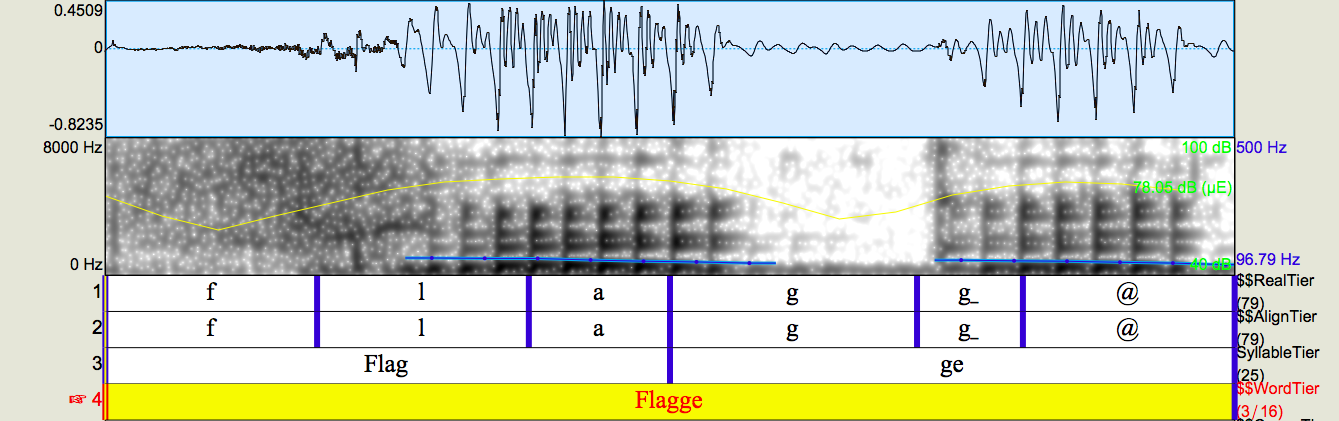
\includegraphics[width=\textwidth]{../../../colloquium/2SH05_FGMB1_527-flagge}
%	\end{figure}
%	\vfill
	
	Manual annotation of LSEs in subset of corpus:\\
	\begin{itemize}
	\item{12 bisyllabic, initial-stress words (word types)
%		\begin{itemize}
%		\item{Bisyllabic}
%		\item{Stress on initial syllable}
%		\end{itemize}
	}
	\item{Word utterances (tokens) extracted automatically}
	\item{%\hspace*{20pt} 
	668 tokens from $\sim$55 French speakers}
	\item{\TODO{X} tokens from L1 German speakers assumed to be error-free; not manually annotated}
	\end{itemize}
	
	
\end{frame}

\section{Method}
\subsection{Feature sets}
\begin{frame}
\end{frame}
\subsection{Evaluation method}
\begin{frame}
\end{frame}

\section{Results}
%\subsection{Feature set performance}
\begin{frame}
\end{frame}
%\subsection{Performance on unseen speakers}
\begin{frame}
\end{frame}

\section{Conclusions \& future work}
\begin{frame}
\end{frame}

\end{document}